\documentclass{article}
\usepackage{graphicx,epsfig,times}

\setlength{\oddsidemargin}{-5mm}
\setlength{\evensidemargin}{-5mm}
\setlength{\topmargin}{-5mm}
\setlength{\textheight}{230mm}
\setlength{\textwidth}{175mm}
\setlength{\parskip}{2mm}
\setlength{\parindent}{0mm}
\setlength{\unitlength}{1mm}
\newlength{\leftbox}
\newlength{\rightbox}
\setlength{\leftbox}{25mm}
\setlength{\rightbox}{145mm}


\title{Levenberg-Marquardt minimisation}
\author{Philip F McLauchlan}
\date{}

\begin{document}
\setcounter{tocdepth}{3}
\setcounter{secnumdepth}{3}
\def \Plucker {Pl\"{u}cker }
\def \half    {\frac{1}{2}}

\def \brj {{\scriptstyle (j)}}
\def \brjm {{\scriptstyle (j-1)}}
\def \brjso {{\scriptstyle (j_1)}}
\def \brjp {{\scriptstyle (j')}}
\def \brjst {{\scriptstyle (j_2)}}
\def \brjsot {{\scriptstyle (j_1j_2)}}
\def \brjpsj {{\scriptstyle (j'j)}}
\def \brjsk {{\scriptstyle (jk)}}
\def \brz {{\scriptstyle (0)}}
\def \bro {{\scriptstyle (1)}}
\def \brt {{\scriptstyle (2)}}
\def \brh {{\scriptstyle (3)}}
\def \brk {{\scriptstyle (k)}}
\def \brzz {{\scriptstyle (0;0)}}
\def \brkj {{\scriptstyle (k;j)}}
\def \brkk {{\scriptstyle (k;k)}}
\def \brkkm {{\scriptstyle (k;k-1)}}
\def \brkmkm {{\scriptstyle (k-1;k-1)}}
\def \brkm {{\scriptstyle (k-1)}}
\def \brko {{\scriptstyle (k+1)}}
\def \broo {{\scriptstyle (11)}}
\def \brot {{\scriptstyle (12)}}
\def \brtt {{\scriptstyle (22)}}
\def \brth {{\scriptstyle (23)}}
\def \brhh {{\scriptstyle (33)}}
\def \brjj {{\scriptstyle (jj)}}
\def \brkk {{\scriptstyle (kk)}}
\def \brmm {{\scriptstyle (k-1\:k-1)}}
\def \brnm {{\scriptstyle (k-2\:k-1)}}
\def \brmk {{\scriptstyle (k-1\:k)}}

\def \inv {^{-1}}
\def \tr {^{\top}}
\def \trinv {^{-\top}}
\def \chol {{\mbox{Chol}}}
\def \Fac {{\mbox{Fac}}}
\def \redun {_{\mbox{red}}}
\def \svd {{\mbox{SVD}}}
\def \kw {k_{\mbox{w}}}

\def \com {c=1,\ldots,m}
\def \jok {j=1,\ldots,k}
\def \ion {i=1,\ldots,n}
\def \loq {l=1,\ldots,q}

\def \Rm     {R}
\def \Ricj  {R_{ic}(j)}
\def \Riok  {R_{i1}(k)}
\def \Rimk  {R_{im}(k)}
\def \Rick  {R_{ic}(k)}
\def \Rock  {R_{1c}(k)}
\def \Rnck  {R_{nc}(k)}

\def \Pff   {P_{ff}}

\def \Pdd   {P_{dd}}
\def \Pcd   {P_{cd}}
\def \Pcc   {P_{cc}}
\def \Pcf   {P_{cf}}
\def \Pfc   {P_{fc}}
\def \Pcl   {P_{cl}}
\def \Pdc   {P_{dc}}
\def \Plc   {P_{lc}}
\def \Pdf   {P_{df}}
\def \Pfd   {P_{fd}}
\def \Pdl   {P_{dl}}
\def \Pld   {P_{ld}}
\def \Pll   {P_{ll}}
\def \Plf   {P_{lf}}
\def \Pfl   {P_{fl}}

\def \Acc    {A_{cc}}
\def \Acl    {A_{cl}}
\def \Alc    {A_{lc}}
\def \Acd    {A_{cd}}
\def \Adc    {A_{dc}}
\def \Acf    {A_{cf}}
\def \Afc    {A_{fc}}
\def \Aff    {A_{ff}}
\def \Affj   {\Aff(j)}
\def \Affk   {\Aff(k)}
\def \Affo   {A_{ff\:1}}
\def \Affm   {A_{ff\:m}}
\def \Affc   {A_{ff\:c}}
\def \Add    {A_{dd}}
\def \Addo   {A_{dd\:1}}
\def \Addk   {\Add(k)}
\def \Addj   {\Add(j)}
\def \Adf    {A_{df}}
\def \Adfoo  {A_{df\:1}(1)}
\def \Adfok  {A_{df\:1}(k)}
\def \Adfmo  {A_{df\:m}(1)}
\def \Adfmk  {A_{df\:m}(k)}
\def \Adfcj  {A_{df\:c}(j)}
\def \Adfck  {A_{df\:c}(k)}
\def \Adfo   {\Adf(1)}
\def \Adfj   {\Adf(j)}
\def \Adfk   {\Adf(k)}
\def \Afd    {A_{fd}}
\def \Afdk   {\Afd(k)}
\def \Afdj   {\Afd(j)}
\def \Adl    {A_{dl}}
\def \Adlo   {\Adl(1)}
\def \Adlj   {\Adl(j)}
\def \Adlk   {\Adl(k)}
\def \Adloo  {A_{dl\:1}(1)}
\def \Adlno  {A_{dl\:n}(1)}
\def \Adlok  {A_{dl\:1}(k)}
\def \Adlnk  {A_{dl\:n}(k)}
\def \Adlij  {A_{dl\:i}(j)}
\def \Adlik  {A_{dl\:i}(k)}
\def \Ald    {A_{ld}}
\def \Aldk   {\Ald(k)}
\def \Aldj   {\Ald(j)}
\def \All    {A_{ll}}
\def \Allk   {\All(k)}
\def \Allo   {A_{ll\:1}}
\def \Alln   {A_{ll\:n}}
\def \Alli   {A_{ll\:i}}
\def \Alf    {A_{lf}}
\def \Afl    {A_{fl}}
\def \Aflicj {A_{fl\:ic}(j)}
\def \Aflj   {\Afl(j)}
\def \Aflk   {\Afl(k)}
\def \Aflic  {A_{fl\:ic}}

\def \Fff    {F_{ff}}
\def \Fdd    {F_{dd}}
\def \Fll    {F_{ll}}

\def \hvec  {{\bf h}}
\def \fvec  {{\bf f}}
\def \kvec  {{\bf k}}
\def \pvec  {{\bf p}}
\def \hicj  {\hvec_{ic}(j)}
\def \tvec  {{\bf t}}
\def \Tvec  {{\bf T}}
\def \Xvec  {{\bf X}}
\def \Pvec  {{\bf P}}
\def \xvec  {{\bf x}}
\def \yvec  {{\bf y}}
\def \zvec  {{\bf z}}
\def \xhat  {\hat{\bf x}}
\def \yhat  {\hat{\bf y}}
\def \zhat  {\hat{\bf z}}
\def \vecz  {{\bf 0}}
\def \matz  {0}
\def \matu  {1}
\def \bvec  {{\bf b}}
\def \rvec  {{\bf r}}
\def \cvec  {{\bf c}}
\def \Rvec  {{\bf R}}
\def \Fvec  {{\bf F}}
\def \Lvec  {{\bf L}}

\def \RCW    {{R}}
\def \TCW    {{\Tvec}}

\def \beginm   {\left(\!\!\begin{array}}
\def \endm     {\end{array}\!\!\right)}

\def \uvec    {{\bf u}}
\def \vvec    {{\bf v}}
\def \wvec    {{\bf w}}
\def \wvecicj {\wvec_{ic}(j)}

\def \avec {{\bf a}}
\def \ahat  {\hat{\bf a}}
\def \af   {\avec_f}
\def \afc  {\avec_{f\:c}}
\def \afo  {\avec_{f\:1}}
\def \afm  {\avec_{f\:m}}
\def \afk  {\avec_f(k)}
\def \ad   {\avec_d}
\def \adj  {\avec_d(j)}
\def \adk  {\avec_d(k)}
\def \ado  {\avec_d(1)}
\def \adk  {\avec_d(k)}
\def \al   {\avec_l}
\def \ali  {\avec_{l\:i}}
\def \alo  {\avec_{l\:1}}
\def \aln  {\avec_{l\:n}}
\def \alk  {\avec_l(k)}
\def \alik {\avec_{l\:i}(k)}
\def \alok {\avec_{l\:1}(k)}
\def \alnk {\avec_{l\:n}(k)}
\def \ac   {\avec_c}
\def \acl  {\avec_{c\:l}}
\def \aco  {\avec_{c\:1}}
\def \acq  {\avec_{c\:q}}
\def \ack  {\avec_c(k)}

\def \nvec {{\bf n}}
\def \qvec {{\bf q}}
\def \lvec {{\bf l}}
\def \lhat {\hat{\bf l}}

\def \xvecfc {\xvec_{f\:c}}
\def \xvecfo {\xvec_{f\:1}}
\def \xvecfm {\xvec_{f\:m}}
\def \xvecd  {\xvec_d}
\def \xvecdj {\xvec_d(j)}
\def \xvecdo {\xvec_d(1)}
\def \xvecdk {\xvec_d(k)}
\def \xvecl  {\xvec_l}
\def \xvecli {\xvec_{l\:i}}
\def \xveclo {\xvec_{l\:1}}
\def \xvecln {\xvec_{l\:n}}
\def \xveccl {\xvec_{c\:l}}
\def \xvecco {\xvec_{c\:1}}
\def \xveccq {\xvec_{c\:q}}

\def \xhatfc {\xhat_{f\:c}}
\def \xhatfcz {\xhat_{f\:c0}}
\def \xhatdjz {\xhat_{d\:0}(j)}
\def \xhatdkz {\xhat_{d\:0}(k)}
\def \xhatdj {\xhat_d(j)}
\def \xhatli {\xhat_{l\:i}}
\def \xhatliz {\xhat_{l\:i0}}
\def \xhatcl {\xhat_{c\:l}}
\def \xhatclz {\xhat_{c\:l0}}

\def \Pffcz {P_{ff\:c0}}
\def \Pddjz {P_{dd\:0}(j)}
\def \Pddkz {P_{dd\:0}(k)}
\def \Plliz {P_{ll\:i0}}
\def \Pcclz {P_{cc\:l0}}

\def \Hficj {H_{f\:ic}(j)}
\def \Hdicj {H_{d\:ic}(j)}
\def \Hdick {H_{d\:ic}(k)}
\def \Hlicj {H_{l\:ic}(j)}
\def \Hcicj {H_{c\:ic}(j)}
\def \Hfick {H_{f\:ic}(k)}
\def \Hlick {H_{l\:ic}(k)}
\def \Hlock {H_{l\:1c}(k)}
\def \Hlnck {H_{l\:nc}(k)}

\def \nuvec {\mbox{\boldmath $\nu$}}
\def \nuvecicj {\mbox{\boldmath $\nu$}_{ic}(j)}
\def \nuvecick {\mbox{\boldmath $\nu$}_{ic}(k)}
\def \lambdavec {\mbox{\boldmath $\lambda$}}
\def \lambdahat  {\hat{\lambdavec}}

\def \sumcm {\sum_{c=1}^m}
\def \sumin {\sum_{i=1}^n}
\def \sumjk {\sum_{j=1}^k}

\def \XvW   {\Xvec_{{\rm W}}}
\def \XvWo  {\Xvec_{{\rm W}1}}
\def \XvWt  {\Xvec_{{\rm W}2}}
\def \XvWi  {\Xvec_{{\rm W}\:i}}
\def \XvWio {\Xvec_{{\rm W}\:i1}}
\def \XvWit {\Xvec_{{\rm W}\:i2}}
\def \XW    {X_{{\rm W}}}
\def \YW    {Y_{{\rm W}}}
\def \ZW    {Z_{{\rm W}}}
\def \XvC   {\Xvec_{{\rm C}}}
\def \XC    {X_{{\rm C}}}
\def \YC    {Y_{{\rm C}}}
\def \ZC    {Z_{{\rm C}}}
\def \xvI   {\xvec_{{\rm I}}}
\def \xvIi  {\xvec_{{\rm I}\:i}}
\def \xI    {x_{{\rm I}}}
\def \yI    {y_{{\rm I}}}
\def \xIi   {x_{{\rm I}\:i}}
\def \yIi   {y_{{\rm I}\:i}}
\def \zI    {z_{{\rm I}}}

\def \Cov {\rm Cov}

\maketitle

The Levenberg-Marquardt
algorithm~\cite{Marquardt:JSIAM63,Bjorck:96}
is a general non-linear downhill minimisation algorithm
for the case when derivatives of the objective function are known.
It dynamically mixes Gauss-Newton and gradient-descent iterations.
We shall develop the L-M algorithm for a simple
case in our notation, which is derived from Kalman filtering
theory~\cite{BarShalom:Fortmann:88}. The Ravl implementation of
Levenberg-Marquardt will then be presented. Let the unknown parameters be
represented by the vector $\xvec$, and let noisy measurements of
$\xvec$ be made:
\begin{equation}
 \zvec\brj = \hvec(j;\xvec) + \wvec\brj,\;\;\jok
 \label{measure_equation}
\end{equation}
where $\hvec\brj$ is a measurement function and $\wvec\brj$ is zero-mean
noise with covariance $N\brj$. Since we are describing an iterative
minimization algorithm, we shall assume that we have already obtained
an estimate $\xhat^-$ of $\xvec$.
Then the maximum likelihood solution for a new estimate $\xhat$ minimizes
\begin{equation}
 \chi^2(\xhat) = \sumjk (\zvec\brj-\hvec(j;\xhat))\tr N\brj\inv (\zvec\brj-\hvec(j;\xhat)).
 \label{chi2-def}
\end{equation}
We form a quadratic approximation to $\chi^2(.)$ around $\xhat^-$, and minimize
this approximation to $\chi^2(.)$ to obtain a new estimate $\xhat^+$.
In general we can write such a quadratic approximation as
\[ \chi^2(\xvec) \approx a - 2\avec\tr(\xvec-\xhat^-) + (\xvec-\xhat^-)\tr A (\xvec-\xhat^-)
\]
for scalar $a$, vectors $\avec$, $\bvec$ and matrices $A$, $B$.
Note that here and in equation~(\ref{chi2-def}) the signs and factors of two
are chosen WLOG to simplify the resulting expressions for the solution.
Differentiating, we obtain
\[
 \frac{\partial \chi^2}{\partial \xvec} = - 2\avec + 2A(\xvec-\xhat^-), \;\;\;\;
\]
\[
 \frac{\partial^2 \chi^2}{\partial \xvec^2} = 2A, \;\;\;\;
\]
At the minimum point $\xhat$ we have $\partial \chi^2/\partial \xvec=\vecz$
which means that
\begin{equation}
 A (\xhat^+-\xhat^-) = \avec.
 \label{chi2-min}
\end{equation}
Thus we need to obtain $\avec$ and $A$ to compute the update.
We now consider the form of $\chi^2(.)$ in~(\ref{chi2-def}).
Writing the Jacobian of $\hvec(j,\xvec)$ as
\[ H\brj=\frac{\partial \hvec\brj}{\partial \xvec},
\]
we have
\begin{eqnarray}
 \frac{\partial \chi^2}{\partial \xvec} &=& -2\sumjk H\brj\tr N\brj\inv (\zvec\brj-\hvec(j;\xvec)), \label{chi2p-def} \\
 \frac{\partial^2 \chi^2}{\partial \xvec^2} &=& 2\sumjk H\brj\tr N\brj\inv H\brj - 2\sumjk \left(\frac{\partial H\brj}{\partial \xvec}\right)\tr N\brj\inv (\zvec\brj-\hvec(j;\xvec)) \nonumber \\
            &\approx& 2\sumjk H\brj\tr N\brj\inv H\brj, \label{chi2pp-def}
\end{eqnarray}
In the last formula for $\partial^2 \chi^2/\partial \xvec^2$, the terms
involving the second derivatives of $\hvec\brj(.)$
have been omitted. This is done because these terms are
generally much smaller and can in practice be omitted, as well as because
the second derivatives are more difficult and complex to compute than the
first derivatives.

Now we solve the above equations for $\avec$ and $A$ given
the values of function $\hvec\brj$ and the Jacobian $H\brj$
evaluated at the previous estimate $\xhat^-$.
We have immediately
\[ A = \sumjk H\brj\tr N\brj\inv H\brj.
\]
We now write the {\em innovation} vectors $\nuvec\brj$ as
\[ \nuvec\brj = \zvec\brj - \hvec(j;\xhat^-)
\]
Then we have
\begin{equation}
 \avec = \sumjk H\brj\tr N\brj\inv \nuvec\brj \label{a-solved}
\end{equation}
Combining equations~(\ref{chi2-min}) and~(\ref{a-solved}) we
obtain the linear system
\begin{equation}
 A (\xhat^+ - \xhat^-) = \avec = \sumjk H\brj\tr N\brj\inv \nuvec\brj
 \label{LM_update}
\end{equation}
to be solved for the adjustment $\xhat^+ - \xhat^-$.
The covariance of the state is
\[ P = A\inv.
\]

The update~(\ref{LM_update}) may be repeated,
substituting the new $\xhat^+$ as $\xhat^-$, and
improving the estimate until convergence is achieved according to some
criterion. Levenberg-Marquardt modifies this updating procedure by
adding a value $\lambda$ to the diagonal elements of the linear system matrix
before inverting it to obtain the update.
$\lambda$ is reduced if the last iteration gave
an improved estimate, i.e. if $\chi^2$ was reduced, and increased if $J$
increased, in which case the estimate of $\xvec$ is reset to the
estimate before the last iteration. It is this that allows the algorithm
to smoothly switch between Gauss-Newton (small $\lambda$) and gradient
descent (large $\lambda$).

This version is a generalization
of Levenberg-Marquardt as it is normally presented
(e.g.~\cite{Press:etal:88}) in that we incorporate vector measurements
$\zvec\brj$ with covariances $N\brj$, rather than scalar measurements
with variances. The full algorithm is as follows:
\begin{enumerate}
 \item Start with a prior estimate $\xhat^-$ of $\xvec$. Initialize $\lambda$
        to some starting value, e.g. 0.001.
 \item Compute the updated estimate $\xhat^+$ by solving the linear
        system~(\ref{LM_update}) for the adjustment, having first added
        $\lambda$ to each diagonal element of $A$.
 \item Compute the least-squares residuals $\chi^2(\xhat^-)$ and $\chi^2(\xhat^+)$
        from~(\ref{chi2-def}).
 \begin{enumerate}
  \item If $\chi^2(\xhat^+)<\chi^2(\xhat^-)$, reduce $\lambda$ by a specified factor
        (say 10), set $\xhat^-$ to $\xhat^+$, and return to step 2.
  \item Otherwise, the update failed to reduce the residual, so increase
        $\lambda$ by a factor (say 10), forget the updated $\xhat^+$ and
        return to step 2.
 \end{enumerate}
\end{enumerate}
The algorithm continues until some pre-specified termination criterion
has been met, such as a small change to the state vector, or a limit on
the number of iterations.

If the measurements $\zvec\brj$ are unbiased and normally distributed,
the residual $\chi^2(\xhat^+)$ is a $\chi^2$ random variable, and testing
the value of $\chi^2$ against a $\chi^2$ distribution is a good way
of checking that the measurement noise model is reasonable.
The number of degrees of freedom (DOF) of the $\chi^2$ distribution
can be determined as the total size of the measurement vectors,
minus the size of the state.
If the $SIZE(.)$ function returns the dimension of its vector
argument, then the degrees of freedom may be computed as
\begin{equation}
 DOF = \sumjk SIZE(\zvec\brj) - SIZE(\xvec).
 \label{LM_DOF}
\end{equation}

\subsection{Robust observations}
An important drawback of standard least-squares algorithm such as
Levenberg-Marquardt is that they assume that all observations are correct.
Various types of estimators have been successfully used to deal with
the presence of outliers in the data.
Examples are least median-of-squares, RANSAC and Hough transform estimators.
These estimators involve a radical redesign of the measurement error model.
We employ what is probably
the simplest method of ``robustifying'' the standard Gaussian error model.
The robust error model used here assumes that the errors follow a
distribution combining a narrow ``inlier'' Gaussian with a wide ``outlier''
Gaussian, as shown for a one-dimensional distribution in
Figure~\ref{gauss_mix}.
\begin{figure}
% \centerline{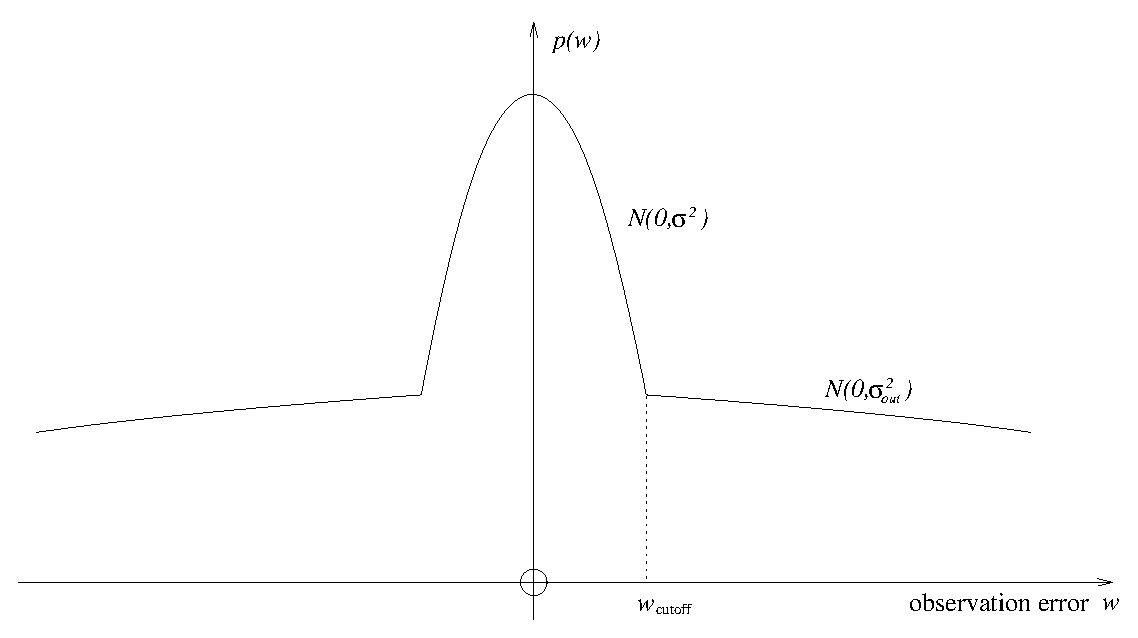
\includegraphics[width=150mm]{gauss_mix.ps}}
 \centerline{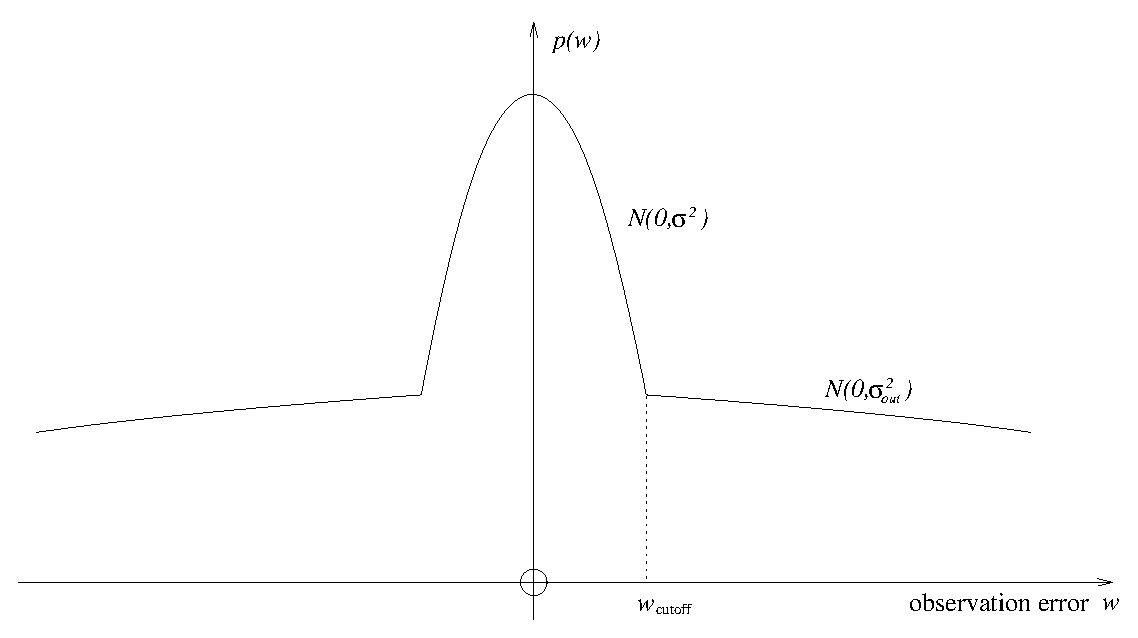
\epsfig{file=gauss_mix.ps,width=150mm}}
  \caption{The error model used to model outliers in the observations
	incorporated in robust Levenberg-Marquardt,
	a combination of a narrow inlier Gaussian with
	variance $\sigma^2$, and wide Gaussian for outliers with
	variance $\sigma_{\rm out}^2$. Both distributions on the
	observation error $w$ have zero mean. The inlier and outlier
	Gaussians are scaled so that they meet continuously at a specific
	error value $w_{\rm cutoff}$, which is effectively an upper error
	threshold for observations to be treated as inliers.}
 \label{gauss_mix}
\end{figure}
The distribution is a function of the observation error\footnote{The innovation
$\nuvec$ is the observation error relative to that computed from the
{\em estimated} state: $\nuvec = \zvec - \hvec(\xhat)$.}
$\wvec = \zvec - \hvec(\xvec)$.
The relative vertical scaling of the two Gaussians is chosen so that the
two distribution functions are equal at a chosen point $w_{\rm cutoff}$.

For a general multi-dimensional observation, we have a inverse covariance
matrix $N\inv$ for the inlier distribution.
We restrict the outlier distribution $N_{\rm out}\inv$ to be a rescaled version
of the inlier distribution, so that
\[ N_{\rm out}\inv = \frac{1}{K} N\inv
\]
for some value $K>1$. We then choose a threshold $\chi_{\rm cutoff}^2$
on the value of the normalised squared error $\chi^2$ for switching between
the two distributions. The probability distribution function is therefore
\[ p(\wvec) = \left\{ \begin{array}{ll} e^{-\wvec\tr N\inv \wvec} &
    \mbox{if}\;\;\;\wvec\tr N\inv \wvec < \chi_{\rm cutoff}^2\;\;\mbox{(inlier)} \\&\\
		 e^{(K\inv -1)\chi_{\rm cutoff}^2} e^{-\wvec\tr N_{\rm out}\inv \wvec}
  & \mbox{otherwise (outlier)} \end{array} \right.
\]
The scaling of the outlier distribution is chosen so that the two distributions
are correctly aligned at the chosen cutoff point $\chi_{\rm cutoff}^2$.
This leads directly to the correct ``compensation'' value for the likelihood
function $(K\inv - 1)\chi_{\rm cutoff}^2$, to be added to the least-squares
residual when the outlier distribution is selected during application
of a minimisation iteration.
Note that each Levenberg-Marquardt observation can be chosen as robust
or non-robust, and potentially each with a different choice for
covariance scale factor $K$ and squared error threshold $\chi_{\rm cutoff}^2$.

\subsection{Implicit observations}
Equation~\ref{measure_equation} does not encapsulate the most general
form of observation, since it assumes that the observation vector $\zvec$
can be separated explicitly as a function $\hvec(\xvec)$ of the state $\xvec$.
It is sometimes therefore necessary to introduce an implicit observation
equation of the form
\[ \Fvec(\xvec,\zvec-\wvec) = \vecz
\]
where $\wvec$ again represents a random noise vector having covariance $N$.
However with some manipulation and extra computation we can effectively
convert the linearised version of the implicit $\Fvec$-type function into an
explicit $\hvec$-type function, allowing it to be incorporated in the same way.
We linearise $\Fvec(.)$ with respect to $\xvec$ and $\zvec$ around the
estimated state $\xhat$ and observation $\zvec$, assuming
that the noise $\wvec$ is small:
\[ \Fvec(\xvec,\zvec_t) = \Fvec(\xhat,\zvec)
	+ \frac{\partial \Fvec}{\partial \xvec} (\xvec-\xhat)
	- \frac{\partial \Fvec}{\partial \zvec} \wvec = \vecz
\]
where $\xvec$ here represents the true value of the state vector, and $\zvec_t$
is the true observation vector (as opposed to the actually measured vector
$\zvec$), so that $\wvec = \zvec-\zvec_t$.
We identify the following quantities with their equivalents for an $\hvec$-type
observation:
\begin{description}
  \item{The {\bf innovation}} vector is $\nuvec=-\Fvec(\xhat,\zvec)$.
  \item{The {\bf Jacobian}} matrix is
	$H=\frac{\partial \Fvec}{\partial \xvec}$.
  \item{The {\bf noise vector}} is
	$\wvec' = \frac{\partial \Fvec}{\partial \zvec} \wvec$.
  \item{The {\bf noise covariance}} matrix is
	$N' = \frac{\partial \Fvec}{\partial \zvec} N \left(\frac{\partial \Fvec}{\partial \zvec}\right)\tr$.
\end{description}
Extra computation is therefore needed to convert the observation covariance
from $N$ to $N'$. The innovation vector $\nuvec$, Jacobian matrix $H$ and
observation covariance $N'$ are substituted into the Levenberg-Marquardt
algorithm in place of their equivalents for the $\hvec$-type observation.

\bibliographystyle{plain}
\bibliography{active}

\end{document}
